\begin{pastexam}[label={px:ntu-110-comm-dsa-38}]{臺大電信所 110 學年度（B）第 38 題}
（複選；每題 2.5 分，每答錯一個選項倒扣 0.5 分至該題 0 分止）

In this exam,
\begin{itemize}
\item The height of a leaf (in either a tree or heap) is defined as 0.
\item The depth of the root (in either a tree or heap) is defined as 0.
\item The degree of a node (in either a tree or heap) is defined as the number of its children.
\item The size of a tree/heap is defined as the total number of keys (items) it stores.
\item All heaps, unless otherwise specified, are min heaps.
\end{itemize}

Consider a binary search tree that results from successively inserting keys 2, 8, 9, 1, 5, 7, 6, 3, 4 into an initially empty tree. Which of the following statements are true?
\begin{enumerate}[label=\Alph*.]
\item The tree height is 4.
\item Key 8 is prior to key 3 in terms of pre-order traversal.
\item Key 2 is prior to key 7 in terms of post-order traversal.
\item Key 4 is prior to key 5 in terms of in-order traversal.
\item Key 3 and key 9 are siblings.
\end{enumerate}
\end{pastexam}

\begin{pastsoln}
答案是 A、B、D。

依序插入：每個鍵從根往下，比節點小往左、大往右，走到空位就放（資結書第~9.2~節）。
$2$ 是根；$8 > 2$ 放右；$9$ 放 $8$ 的右；$1$ 放 $2$ 的左；$5$：$>2$、$<8$，放 $8$ 的左；$7$：$>2, <8, >5$，
放 $5$ 的右；$6$：$>2, <8, >5, <7$，放 $7$ 的左；$3$：$>2, <8, <5$，放 $5$ 的左；$4$：$>2, <8, <5, >3$，
放 $3$ 的右。
\begin{center}
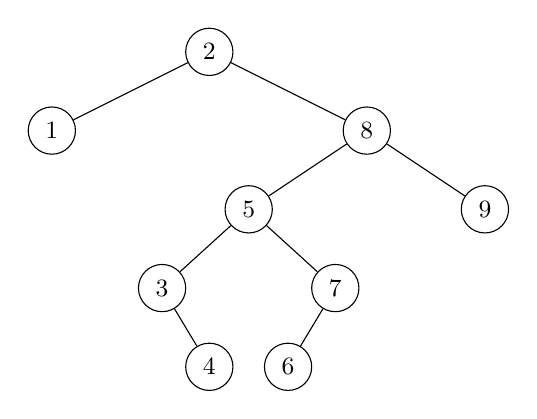
\begin{tikzpicture}[every node/.style={circle,draw,inner sep=1pt,minimum size=6mm,font=\small},level distance=10mm,edge from parent/.style={draw},level 1/.style={sibling distance=40mm},level 2/.style={sibling distance=30mm},level 3/.style={sibling distance=22mm},level 4/.style={sibling distance=12mm}]
\node {2}
  child {node {1}}
  child {node {8}
    child {node {5}
      child {node {3} child[missing] child {node {4}}}
      child {node {7} child {node {6}} child[missing]}}
    child {node {9}}};
\end{tikzpicture}
\end{center}
走訪順序：
\begin{itemize}
\item 前序：$2, 1, 8, 5, 3, 4, 7, 6, 9$
\item 中序：$1, 2, 3, 4, 5, 6, 7, 8, 9$
\item 後序：$1, 4, 3, 6, 7, 5, 9, 8, 2$
\end{itemize}
\begin{itemize}
\item A 對：最長的根到葉路徑是 $2 \to 8 \to 5 \to 3 \to 4$（或 $\to 7 \to 6$），$4$ 條邊。 本卷葉子高度為 $0$，
樹高 $4$。
\item B 對：前序裡 $8$ 是第 $3$ 個，$3$ 是第 $5$ 個。 $3$ 在 $8$ 的子樹裡，前序先印祖先。
\item C 錯：後序最後才印根 $2$，$7$ 在它前面。
\item D 對：中序就是由小到大，$4$ 在 $5$ 前面。
\item E 錯：$3$ 的父節點是 $5$，$9$ 的父節點是 $8$，不是兄弟（$9$ 的兄弟是 $5$）。
\end{itemize}
\end{pastsoln}
